\documentclass{article}

\usepackage[utf8]{inputenc}
\usepackage[letterpaper, total={6in, 9in}]{geometry}
\usepackage{amsmath}
\usepackage{natbib}
\usepackage{wrapfig}
\usepackage{graphicx}
\usepackage{amssymb}
\usepackage{tikz}

\graphicspath{ {./geo1/} }

\title{Geometry 1 - Basis of Geometry}
\author{TSS Math Club}
\date{Oct 2022}

\begin{document}
\large

\maketitle

\section{Parallelism and basic geometry}
\subsection{Parallel lines}
\subsubsection{Parallel postulate}
If a line segment intersects two straight lines forming two interior angles on the same side that are less than two right angles, then the two lines, if extended indefinitely, meet on that side on which the angles sum to less than two right angles.
\subsubsection{Definition}
Two lines in two-dimensional Euclidean space are said to be parallel if they do not intersect.
\subsubsection{Parallel Lines and Transversal}


\tikzset{every picture/.style={line width=0.75pt}} %set default line width to 0.75pt        

\begin{tikzpicture}[x=0.75pt,y=0.75pt,yscale=-1,xscale=1]
%uncomment if require: \path (0,300); %set diagram left start at 0, and has height of 300

%Straight Lines [id:da21139363812284984] 
\draw    (100,102) -- (410.58,103.17) ;
%Straight Lines [id:da7932846415944257] 
\draw    (99.58,199.17) -- (409.58,198.17) ;
%Straight Lines [id:da5509456601565808] 
\draw    (283.58,69.17) -- (183.58,235.17) ;

% Text Node
\draw (279,81) node [anchor=north west][inner sep=0.75pt]   [align=left] {1};
% Text Node
\draw (251,82) node [anchor=north west][inner sep=0.75pt]   [align=left] {2};
% Text Node
\draw (239,105) node [anchor=north west][inner sep=0.75pt]   [align=left] {3};
% Text Node
\draw (266,105) node [anchor=north west][inner sep=0.75pt]   [align=left] {4};
% Text Node
\draw (217,180) node [anchor=north west][inner sep=0.75pt]   [align=left] {5};
% Text Node
\draw (191,180) node [anchor=north west][inner sep=0.75pt]   [align=left] {6};
% Text Node
\draw (183,203) node [anchor=north west][inner sep=0.75pt]   [align=left] {7};
% Text Node
\draw (207,204) node [anchor=north west][inner sep=0.75pt]   [align=left] {8};


\end{tikzpicture}

\begin{itemize}
    \item Corresponding angles are equal ($\angle 1=\angle 5$)
    \item Alternate angles are equal ($\angle 3=\angle 5$)
    \item Co-interior angles are supplementary to each other ($\angle 4+\angle 5$=$180^{\circ}$)
\end{itemize}

\subsection{Parallel is transitive}

\begin{minipage}{.6\linewidth}
\tikzset{every picture/.style={line width=0.75pt}} %set default line width to 0.75pt        

\begin{tikzpicture}[x=0.75pt,y=0.75pt,yscale=-1,xscale=1]
%uncomment if require: \path (0,300); %set diagram left start at 0, and has height of 300

%Straight Lines [id:da21139363812284984] 
\draw    (100,102) -- (410.58,103.17) ;
%Straight Lines [id:da7932846415944257] 
\draw    (99.58,199.17) -- (409.58,198.17) ;
%Straight Lines [id:da5509456601565808] 
\draw    (283.58,69.17) -- (183.58,235.17) ;
%Straight Lines [id:da3298327170129234] 
\draw    (102.58,152.17) -- (412.58,151.17) ;

% Text Node
\draw (279,81) node [anchor=north west][inner sep=0.75pt]   [align=left] {1};
% Text Node
\draw (245,133) node [anchor=north west][inner sep=0.75pt]   [align=left] {2};
% Text Node
\draw (218,182) node [anchor=north west][inner sep=0.75pt]   [align=left] {3};


\end{tikzpicture}
\end{minipage}
\hfill
\begin{minipage}{.3\linewidth}
$$\begin{array}{l}
\because k / / l \\
\therefore \angle 1=\angle 2 \\
\because l / / m \\
\therefore \angle 2=\angle 3 \\
\therefore \angle 1=\angle 3 \\
\therefore k / / m
\end{array}$$
\end{minipage}

\subsection{Sum of the interior angles of a triangle is $180^\circ$}
\begin{minipage}{.45\linewidth}
    

\tikzset{every picture/.style={line width=0.75pt}} %set default line width to 0.75pt        

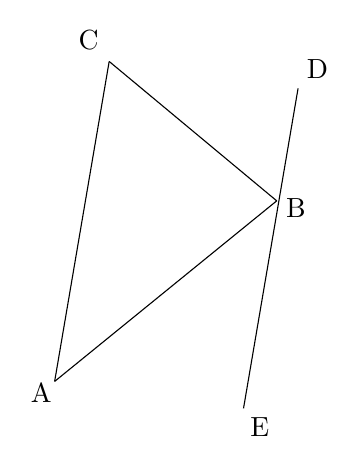
\begin{tikzpicture}[x=0.75pt,y=0.75pt,yscale=-1,xscale=1]
%uncomment if require: \path (0,300); %set diagram left start at 0, and has height of 300

%Straight Lines [id:da0699676175520938] 
\draw    (201,82) -- (281.72,149.17) ;
%Straight Lines [id:da030285405179883762] 
\draw    (201,82) -- (174.72,236.17) ;
%Straight Lines [id:da34572122009938444] 
\draw    (281.72,149.17) -- (174.72,236.17) ;
%Straight Lines [id:da5559272769704977] 
\draw    (292,95) -- (265.72,249.17) ;

% Text Node
\draw (162,236) node [anchor=north west][inner sep=0.75pt]   [align=left] {A};
% Text Node
\draw (285,147) node [anchor=north west][inner sep=0.75pt]   [align=left] {B};
% Text Node
\draw (185,66) node [anchor=north west][inner sep=0.75pt]   [align=left] {C};
% Text Node
\draw (295,80) node [anchor=north west][inner sep=0.75pt]   [align=left] {D};
% Text Node
\draw (267.72,252.17) node [anchor=north west][inner sep=0.75pt]   [align=left] {E};


\end{tikzpicture}
\end{minipage}
\hfill
\begin{minipage}{.45\linewidth}
    Draw line DE through $\mathrm{B}$ such that $\mathrm{DE} / / \mathrm{AC}$
$$
\begin{aligned}
\because & A C / / D E \\
\therefore & \angle A=\angle A B E \\
& \angle B=\angle C B D \\
\therefore & \angle A+\angle B+\angle C \\
& =\angle C B D+\angle C B A+\angle A B E \\
& =180^{\circ}
\end{aligned}
$$
\end{minipage}
\subsection{Sum of interior angles of a n-gon is $(n-2)180^\circ$}
\begin{minipage}{.5\linewidth}
    



\tikzset{every picture/.style={line width=0.75pt}} %set default line width to 0.75pt        

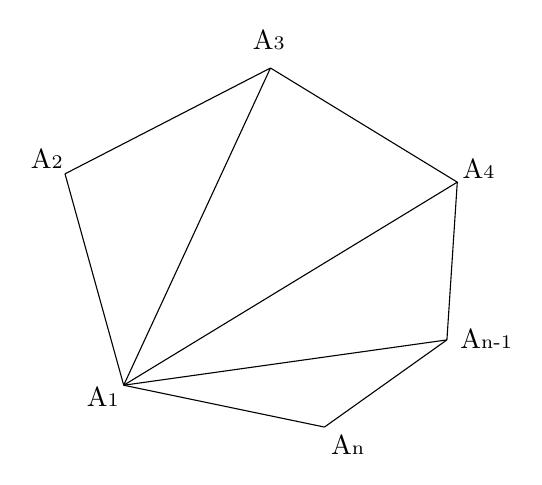
\begin{tikzpicture}[x=0.75pt,y=0.75pt,yscale=-1,xscale=1]
%uncomment if require: \path (0,300); %set diagram left start at 0, and has height of 300

%Straight Lines [id:da8100209405163055] 
\draw    (171.72,114.16) -- (200,216) ;
%Straight Lines [id:da5194616266478809] 
\draw    (171.72,114.16) -- (270.72,63.16) ;
%Straight Lines [id:da8019767973952356] 
\draw    (270.72,63.16) -- (360.72,118.16) ;
%Straight Lines [id:da47367808311702664] 
\draw    (200,216) -- (296.72,236.16) ;
%Straight Lines [id:da7032796995738642] 
\draw    (296.72,236.16) -- (355.72,194.16) ;
%Straight Lines [id:da8988664824053545] 
\draw    (360.72,118.16) -- (355.72,194.16) ;
%Straight Lines [id:da024792389830001982] 
\draw    (200,216) -- (360.72,118.16) ;
%Straight Lines [id:da8434062186507831] 
\draw    (200,216) -- (355.72,194.16) ;
%Straight Lines [id:da6287048649240963] 
\draw    (200,216) -- (270.72,63.16) ;

% Text Node
\draw (181,216) node [anchor=north west][inner sep=0.75pt]   [align=left] {A{\scriptsize 1}};
% Text Node
\draw (154,101) node [anchor=north west][inner sep=0.75pt]   [align=left] {A{\scriptsize 2}};
% Text Node
\draw (261,44) node [anchor=north west][inner sep=0.75pt]   [align=left] {A{\scriptsize 3}};
% Text Node
\draw (362,106) node [anchor=north west][inner sep=0.75pt]   [align=left] {A{\scriptsize 4}};
% Text Node
\draw (361,188) node [anchor=north west][inner sep=0.75pt]   [align=left] {A{\scriptsize n-1}};
% Text Node
\draw (298.72,239.16) node [anchor=north west][inner sep=0.75pt]   [align=left] {A{\scriptsize n}};


\end{tikzpicture}
\end{minipage}
\hfill
\begin{minipage}{.5\linewidth}
    It can be partitioned into n-2 triangles. 
Since the sum of interior angles of a n-gon is the sum of all the interior angles of the triangles, by the theorem above, the interior angles = number of triangles $\times 180^\circ$ or 
$(n-2) \times 180^\circ$.

\end{minipage}

\subsection{Exterior angle theorem}
\begin{minipage}{.5\linewidth}


\tikzset{every picture/.style={line width=0.75pt}} %set default line width to 0.75pt        

\begin{tikzpicture}[x=0.75pt,y=0.75pt,yscale=-1,xscale=1]
%uncomment if require: \path (0,300); %set diagram left start at 0, and has height of 300

%Straight Lines [id:da4962210423643947] 
\draw    (109.72,221.16) -- (424.72,221.16) ;
%Straight Lines [id:da6506366962747094] 
\draw    (224.72,98.16) -- (109.72,221.16) ;
%Straight Lines [id:da04022560611735915] 
\draw    (224.72,98.16) -- (275.72,220.16) ;

% Text Node
\draw (103,225) node [anchor=north west][inner sep=0.75pt]   [align=left] {A};
% Text Node
\draw (269.22,224.16) node [anchor=north west][inner sep=0.75pt]   [align=left] {B};
% Text Node
\draw (228,80) node [anchor=north west][inner sep=0.75pt]   [align=left] {C};
% Text Node
\draw (122,204) node [anchor=north west][inner sep=0.75pt]   [align=left] {a};
% Text Node
\draw (253,202) node [anchor=north west][inner sep=0.75pt]   [align=left] {b};
% Text Node
\draw (217,114) node [anchor=north west][inner sep=0.75pt]   [align=left] {c};
% Text Node
\draw (279,203) node [anchor=north west][inner sep=0.75pt]   [align=left] {d};


\end{tikzpicture}

    
\end{minipage}
\hfill
\begin{minipage}{.5\linewidth}
$$    \begin{aligned}
\because a+b+c=180^{\circ} \\
\quad b+d=180^{\circ} \\
\therefore a+c-d=0 \\
\text { or } a+c=d
\end{aligned}$$
\end{minipage}
\subsection{Another problem}

Given $\mathrm{AB} / / \mathrm{CD}, \mathrm{AE}$ bisect $\mathrm{BAC}, \mathrm{CE}$ bisect $\mathrm{ACD}$, prove $\mathrm{AE}$ perpendicular to $\mathrm{CE}$.

\tikzset{every picture/.style={line width=0.75pt}} %set default line width to 0.75pt        

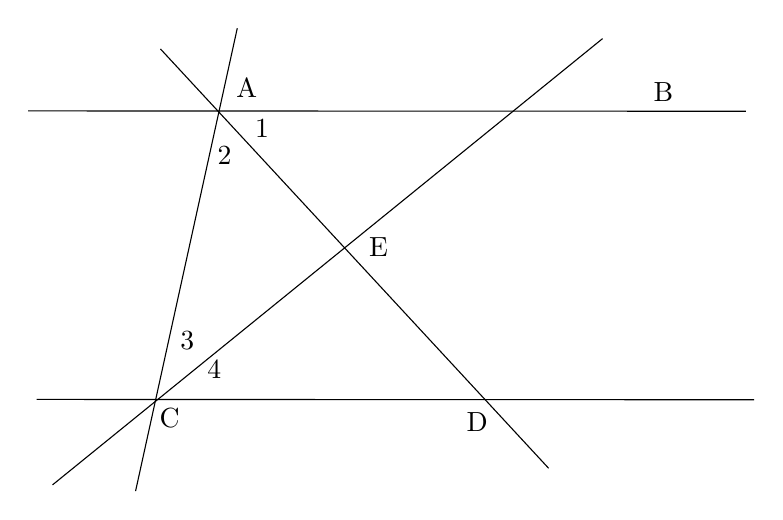
\begin{tikzpicture}[x=0.75pt,y=0.75pt,yscale=-1,xscale=1]
%uncomment if require: \path (0,300); %set diagram left start at 0, and has height of 300

%Straight Lines [id:da39103308479814713] 
\draw    (100,101) -- (445.72,101.16) ;
%Straight Lines [id:da7355224615195692] 
\draw    (104,240) -- (449.72,240.16) ;
%Straight Lines [id:da0002054298491724893] 
\draw    (200.72,61.16) -- (151.72,284.16) ;
%Straight Lines [id:da1159047198742802] 
\draw    (376.72,66.16) -- (111.72,281.16) ;
%Straight Lines [id:da31819404476733126] 
\draw    (163.72,71.16) -- (350.72,273.16) ;

% Text Node
\draw (199,84) node [anchor=north west][inner sep=0.75pt]   [align=left] {A};
% Text Node
\draw (400,86) node [anchor=north west][inner sep=0.75pt]   [align=left] {B};
% Text Node
\draw (162,243) node [anchor=north west][inner sep=0.75pt]   [align=left] {C};
% Text Node
\draw (310,245) node [anchor=north west][inner sep=0.75pt]   [align=left] {D};
% Text Node
\draw (263,161) node [anchor=north west][inner sep=0.75pt]   [align=left] {E};
% Text Node
\draw (208,104) node [anchor=north west][inner sep=0.75pt]   [align=left] {1};
% Text Node
\draw (190,117) node [anchor=north west][inner sep=0.75pt]   [align=left] {2};
% Text Node
\draw (172,206) node [anchor=north west][inner sep=0.75pt]   [align=left] {3};
% Text Node
\draw (185,220) node [anchor=north west][inner sep=0.75pt]   [align=left] {4};


\end{tikzpicture}\\


$$
\begin{aligned}
& \because A E, C E \text { are bisectors } \\
& \therefore \angle 2=\frac{\angle B A C}{2} \\
& \text { and } \angle 3=\frac{\angle A C D}{2} \\
& \therefore \angle 2+\angle 3=\frac{\angle B A C+\angle A C D}{2} \\
& \because A B / / C D \\
& \therefore \angle B A C+\angle A C D=180^{\circ} \\
& \therefore \angle 2+\angle 3=\frac{\angle B A C+\angle A C D}{2}=\frac{180^{\circ}}{2}=90^{\circ} \\
& \therefore \angle A E C=180^{\circ}-(\angle 2+\angle 3)=90^{\circ}\\
& \therefore \mathrm{AE}\text{ is perpendicular to }  \mathrm{CE}
\end{aligned}
$$
\pagebreak
\section{Congruence}
\subsection{Definition}
The same shape and size.
\subsection{Method to prove congruence}
\subsubsection{5 Methods:}
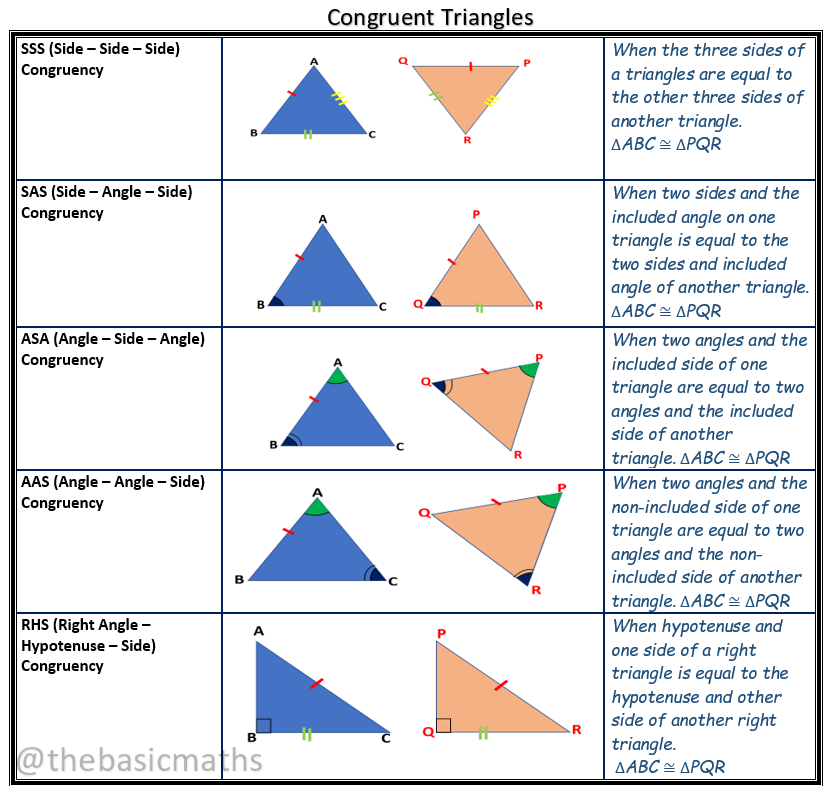
\includegraphics[scale=.5]{congruent-triangles.png}
\subsubsection{How to write in a contest}
In the $\triangle \mathrm{ABC}$ and $\triangle \mathrm{A}^{\prime} \mathrm{B}^{\prime} \mathrm{C}^{\prime}$
$$
\begin{aligned}
& \left\{\begin{array}{l}
\text { Condition } 1 \\
\text { Condition } 2 \\
\text { Condition } 3
\end{array}\right. \\
& \therefore \triangle \mathrm{ABC} \cong \triangle \mathrm{A}^{\prime} \mathrm{B}^{\prime} \mathrm{C}^{\prime}
\end{aligned}
$$
\subsection{Side-Side-Angle (SSA), the ambiguous case}


\tikzset{every picture/.style={line width=0.75pt}} %set default line width to 0.75pt        

\begin{tikzpicture}[x=0.75pt,y=0.75pt,yscale=-1.5,xscale=1.5]
%uncomment if require: \path (0,456); %set diagram left start at 0, and has height of 456

%Straight Lines [id:da7536078114357907] 
\draw    (203.72,34.16) -- (84.72,172.16) ;
%Straight Lines [id:da8068675521405164] 
\draw    (84.72,172.16) -- (184.72,171.16) ;
%Straight Lines [id:da8688445810261354] 
\draw    (203.72,34.16) -- (184.72,171.16) ;
%Straight Lines [id:da0589832509310495] 
\draw    (423.72,33.16) -- (304.72,171.16) ;
%Straight Lines [id:da6036368217646264] 
\draw    (304.72,171.16) -- (404.72,170.16) ;
%Straight Lines [id:da3459836007320729] 
\draw    (423.72,33.16) -- (404.72,170.16) ;
%Straight Lines [id:da31704994457175983] 
\draw    (208.72,209.16) -- (89.72,347.16) ;
%Straight Lines [id:da29956065989182235] 
\draw    (89.72,347.16) -- (238.72,345.16) ;
%Straight Lines [id:da7716237120676077] 
\draw    (208.72,209.16) -- (189.72,346.16) ;
%Straight Lines [id:da0469601268460762] 
\draw    (208.72,209.16) -- (238.72,345.16) ;
%Straight Lines [id:da6549295985369503] 
\draw    (400.72,205.16) -- (281.72,343.16) ;
%Straight Lines [id:da5401188295697685] 
\draw    (281.72,343.16) -- (430.72,341.16) ;
%Straight Lines [id:da20687323955974435] 
\draw    (400.72,205.16) -- (430.72,341.16) ;
%Curve Lines [id:da9622511708823469] 
\draw    (189.72,353.16) .. controls (200.5,364.92) and (217.04,371.88) .. (237.46,352.39) ;
\draw [shift={(238.72,351.16)}, rotate = 135] [color={rgb, 255:red, 0; green, 0; blue, 0 }  ][line width=0.75]    (10.93,-3.29) .. controls (6.95,-1.4) and (3.31,-0.3) .. (0,0) .. controls (3.31,0.3) and (6.95,1.4) .. (10.93,3.29)   ;
\end{tikzpicture}

\pagebreak

\subsubsection{Proof related to the ambiguous case}
Given $\mathrm{AB}=\mathrm{DE}, \mathrm{BC}=\mathrm{EF}$, angle $\mathrm{A}=$ angle $\mathrm{D}>90^{\circ}$, prove triangle $\mathrm{ABC}$ congruent to triangle DEF.



\tikzset{every picture/.style={line width=0.75pt}} %set default line width to 0.75pt        

\begin{tikzpicture}[x=0.75pt,y=0.75pt,yscale=-1,xscale=1]
%uncomment if require: \path (0,456); %set diagram left start at 0, and has height of 456

%Straight Lines [id:da2412202289072125] 
\draw    (99.28,123.87) -- (163.64,231.04) ;
%Straight Lines [id:da0762023899725901] 
\draw    (307.16,233.45) -- (163.64,231.04) ;
%Straight Lines [id:da36331859096149155] 
\draw    (307.16,233.45) -- (99.28,123.87) ;
%Straight Lines [id:da424917208310148] 
\draw    (335.28,125.87) -- (399.64,233.04) ;
%Straight Lines [id:da6245379789708037] 
\draw    (543.16,235.45) -- (399.64,233.04) ;
%Straight Lines [id:da8354045334191129] 
\draw    (543.16,235.45) -- (335.28,125.87) ;

% Text Node
\draw (155,243) node [anchor=north west][inner sep=0.75pt]   [align=left] {A};
% Text Node
\draw (306,244) node [anchor=north west][inner sep=0.75pt]   [align=left] {B};
% Text Node
\draw (86,107) node [anchor=north west][inner sep=0.75pt]   [align=left] {C};
% Text Node
\draw (395,242) node [anchor=north west][inner sep=0.75pt]   [align=left] {D};
% Text Node
\draw (541,244) node [anchor=north west][inner sep=0.75pt]   [align=left] {E};
% Text Node
\draw (318,110) node [anchor=north west][inner sep=0.75pt]   [align=left] {F};


\end{tikzpicture}\\
Extend $CA$ and draw $BX$ perpendicular to $CA$ at $X$\\
Extend $FD$ and draw $EY$ perpendicular to $FD$ at $Y$\\

$$\begin{aligned}
& \because \text { the perpendicular } \\
& \therefore \angle X=\angle Y=90^{\circ} \\
& \because \angle B A C=\angle E D F \\
& \therefore \angle B A X=\angle E D Y \\
& \text { In } \triangle ABX \text { and } \triangle DEY \\
& \left\{\begin{array}{c}
\angle X=\angle Y \\
\angle BAX=\angle EDY \\
A B=D E
\end{array}\right. \\
& \therefore \triangle ABX \cong \triangle DEY(\mathrm{AAS}) \\
& \therefore B X=E Y\\
& \text { In } \triangle CBX \text { and } \triangle FEY \\
& \left\{\begin{array}{l}
B X=E Y \\
B C=E F
\end{array}\right. \\
& \therefore \text { Rt } \triangle CBX \cong \mathrm{Rt} \triangle FEY(\mathrm{HL}) \\
& \therefore \angle C=\angle F \\
& \text { In } \triangle ABC \text { and } \triangle DEF \\
& \left\{\begin{aligned}
\angle C & =\angle F \\
\angle BAC & =\angle EDF \\
A B & =D E
\end{aligned}\right. \\
& \therefore \triangle ABC \cong \triangle DEF(\mathrm{AAS}) \\
&
\end{aligned}
$$
\pagebreak
\subsection{Useful congruencies}
\begin{itemize}
    \item Rotation
    \item Translation
\end{itemize}

\subsection{Properties of congruence}
\begin{itemize}
    \item Equal side length 
    \item Equal angles
\end{itemize}

\subsection{Problems}
\subsubsection{Problem}
Assume $ABD$ and $BCE$ are equilateral triangles, find angle $DFA$.


\tikzset{every picture/.style={line width=0.75pt}} %set default line width to 0.75pt        

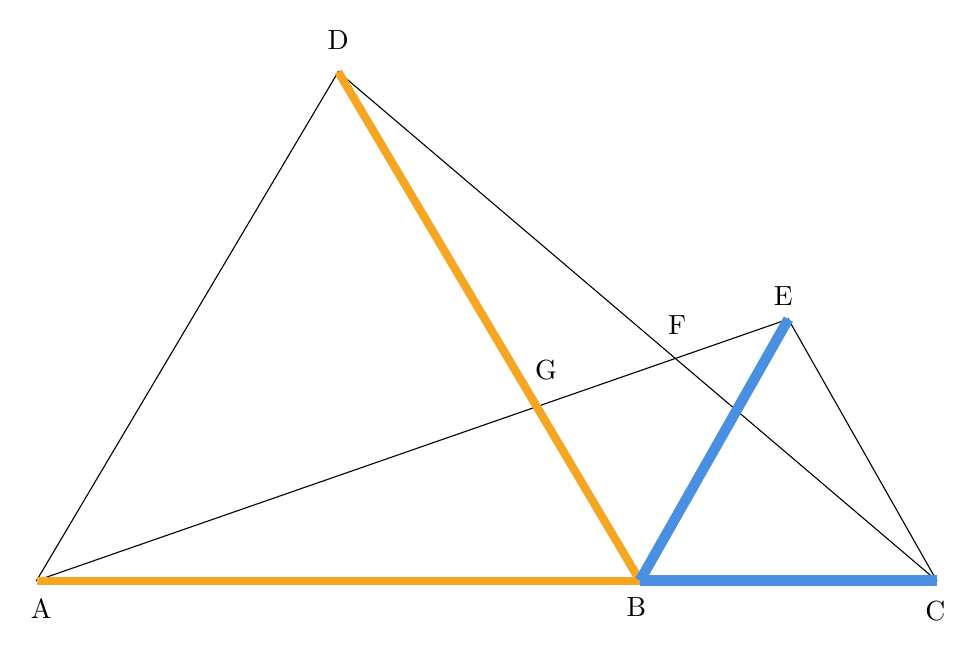
\begin{tikzpicture}[x=0.75pt,y=0.75pt,yscale=-1,xscale=1]
%uncomment if require: \path (0,456); %set diagram left start at 0, and has height of 456

%Shape: Triangle [id:dp28557056970026884] 
\draw   (183.36,112) -- (328.72,357.16) -- (38,357.16) -- cycle ;
%Shape: Triangle [id:dp6204088218917005] 
\draw   (400.22,231.16) -- (471.72,357.16) -- (328.72,357.16) -- cycle ;
%Straight Lines [id:da42886636780202325] 
\draw    (183.36,112) -- (471.72,357.16) ;
%Straight Lines [id:da08024073219320216] 
\draw    (400.22,231.16) -- (38,357.16) ;
%Straight Lines [id:da38494277533771926] 
\draw [color={rgb, 255:red, 245; green, 166; blue, 35 }  ,draw opacity=1 ][line width=3]    (183.36,112) -- (328.72,357.16) ;
%Straight Lines [id:da9375484076382308] 
\draw [color={rgb, 255:red, 245; green, 166; blue, 35 }  ,draw opacity=1 ][line width=3]    (38,357.16) -- (328.72,357.16) ;
%Straight Lines [id:da5007362747375794] 
\draw [color={rgb, 255:red, 74; green, 144; blue, 226 }  ,draw opacity=1 ][line width=3.75]    (328.72,357.16) -- (471.72,357.16) ;
%Straight Lines [id:da989076009762959] 
\draw [color={rgb, 255:red, 74; green, 144; blue, 226 }  ,draw opacity=1 ][line width=3.75]    (400.22,231.16) -- (328.72,357.16) ;

% Text Node
\draw (34,365) node [anchor=north west][inner sep=0.75pt]   [align=left] {A};
% Text Node
\draw (321,364) node [anchor=north west][inner sep=0.75pt]   [align=left] {B};
% Text Node
\draw (465,366) node [anchor=north west][inner sep=0.75pt]   [align=left] {C};
% Text Node
\draw (177,91) node [anchor=north west][inner sep=0.75pt]   [align=left] {D};
% Text Node
\draw (392,214) node [anchor=north west][inner sep=0.75pt]   [align=left] {E};
% Text Node
\draw (341,228) node [anchor=north west][inner sep=0.75pt]   [align=left] {F};
% Text Node
\draw (277,250) node [anchor=north west][inner sep=0.75pt]   [align=left] {G};


\end{tikzpicture}\\
$$\begin{array}{ll}
\because A B D \text { and } B C E \text { are equilateral triangles } & \therefore \angle E A B=\angle C D B=x \\
\therefore A B=B D, B C=B E & \therefore \angle D G A=\angle E A B+\angle D B A \\
\angle A B D=\angle C B E=60^{\circ} & =\angle C D B+\angle D F A=60^{\circ}+x \\
\therefore \angle D B E=180^{\circ}-60^{\circ}-60^{\circ}=60^{\circ} & \therefore \angle \mathrm{DFA}=60^{\circ} \\
\therefore \angle A B E=\angle \mathrm{DBC}=120^{\circ} & \\
\text { In } \triangle \mathrm{ABE} \text { and } \triangle \mathrm{DBC} & \\
\{\mathrm{AB}=\mathrm{DB} & \\
\angle A B E=\angle \mathrm{DBC} & \\
\mathrm{BE}=\mathrm{BC} & \\
\therefore \mathrm{ABE} \cong \triangle \mathrm{DBC}(\mathrm{SAS}) &
\end{array}$$
\pagebreak
\subsubsection{Problem}
$\text { Given } ABCD \text { is a square, and } \angle EAF=45^{\circ} \text {, prove } AE \text { bisect } BEF \text {. }$


\tikzset{every picture/.style={line width=0.75pt}} %set default line width to 0.75pt        

\begin{tikzpicture}[x=0.75pt,y=0.75pt,yscale=-1,xscale=1]
%uncomment if require: \path (0,456); %set diagram left start at 0, and has height of 456

%Shape: Rectangle [id:dp40270396443476963] 
\draw   (198,73.07) -- (497.72,73.07) -- (497.72,359.07) -- (198,359.07) -- cycle ;
%Straight Lines [id:da6518917345863742] 
\draw    (198,73.07) -- (496.72,209.07) ;
%Straight Lines [id:da34344101733280197] 
\draw    (198,73.07) -- (265.72,358.07) ;
%Straight Lines [id:da9392050452094853] 
\draw    (496.72,209.07) -- (265.72,358.07) ;
%Straight Lines [id:da8480244514911197] 
\draw    (198,73.07) -- (55.72,358.07) ;
%Straight Lines [id:da9279966987044268] 
\draw    (55.72,358.07) -- (198,359.07) ;

% Text Node
\draw (193,50) node [anchor=north west][inner sep=0.75pt]   [align=left] {A};
% Text Node
\draw (496,53) node [anchor=north west][inner sep=0.75pt]   [align=left] {B};
% Text Node
\draw (495,371) node [anchor=north west][inner sep=0.75pt]   [align=left] {C};
% Text Node
\draw (191,371) node [anchor=north west][inner sep=0.75pt]   [align=left] {D};
% Text Node
\draw (503,202) node [anchor=north west][inner sep=0.75pt]   [align=left] {E};
% Text Node
\draw (261,371) node [anchor=north west][inner sep=0.75pt]   [align=left] {F};
% Text Node
\draw (46,368) node [anchor=north west][inner sep=0.75pt]   [align=left] {E'};


\end{tikzpicture}\\
\\
$$
\begin{array}{ll}
\text{Extend  CD  to  E'  such that  E' D=BE} \\
\text {Connect E'A } \\
\because A B C D \text { is a square } \\

\therefore A D=A B \quad \\
\angle B=\angle A D E^{\prime}=90^{\circ} \quad \\
\text { In } \triangle A D E^{\prime} \text { and } \triangle A B E \quad  \\
\left\{\begin{array}{c}
\mathrm{AD}=\mathrm{AB} \\
\angle B=\angle A D E \\
\mathrm{DE}^{\prime}=\mathrm{BE}
\end{array}\right. \\
\therefore \triangle A D E^{\prime} \cong \triangle A B E(S A S) \\
\therefore A E^{\prime}=A E \\
\angle \mathrm{AEB}=\angle \mathrm{E}^{\prime} \\
\angle E^{\prime} A D=\angle E A B \\
\therefore \angle E^{\prime} A F=\angle E^{\prime} A D+\angle D A F \\
=\angle E A B+\angle D A F=90^{\circ}-\angle E A F=45^{\circ} \\
\text { In } \triangle A F E^{\prime} \text { and } \triangle A F E \quad  \\
\left\{\begin{array}{c}
\mathrm{AF}=\mathrm{AF} \\
\angle E A F=\angle E^{\prime} A F=45^{\circ} \\
\mathrm{AE}^{\prime}=\mathrm{AE}
\end{array}\right. \\
\therefore \triangle A F E^{\prime} \cong \triangle A F E(\mathrm{SAS}) \\
\therefore \angle A E F=\angle E^{\prime}=\angle A E B \\
\therefore \mathrm{AE} \text { bisect } \mathrm{BEF}
\end{array}
$$
\pagebreak

\subsubsection{Problem}
Given  $AB=BC$  and angle  $ABC=90^{\circ}$, $AD=\sqrt{5}$, $BD=\sqrt{2}$, $DC=3$ , find angle $ADB$.



\tikzset{every picture/.style={line width=0.75pt}} %set default line width to 0.75pt        

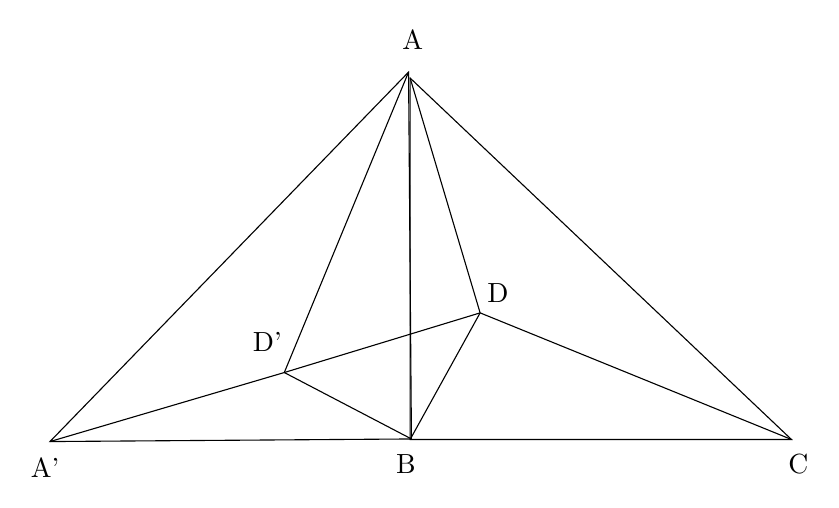
\begin{tikzpicture}[x=0.75pt,y=0.75pt,yscale=-1,xscale=1]
%uncomment if require: \path (0,585); %set diagram left start at 0, and has height of 585

%Shape: Right Triangle [id:dp5392368456885055] 
\draw   (303,155.83) -- (486.72,329.97) -- (303,329.97) -- cycle ;
%Straight Lines [id:da9742494765553811] 
\draw    (303,155.83) -- (336.72,268.97) ;
%Straight Lines [id:da2965189850336305] 
\draw    (336.72,268.97) -- (303,329.97) ;
%Straight Lines [id:da9594379890345373] 
\draw    (336.72,268.97) -- (486.72,329.97) ;
%Shape: Right Triangle [id:dp6408968490039333] 
\draw   (129.48,330.97) -- (302.24,152.97) -- (303.63,329.72) -- cycle ;
%Straight Lines [id:da6174376234301611] 
\draw    (129.48,330.97) -- (242.37,297.71) ;
%Straight Lines [id:da051510717338542955] 
\draw    (242.37,297.71) -- (303.62,329.71) ;
%Straight Lines [id:da2447012279214884] 
\draw    (242.37,297.71) -- (302.24,152.97) ;
%Straight Lines [id:da4682187678291241] 
\draw    (336.72,268.97) -- (242.37,297.71) ;

% Text Node
\draw (298,131.83) node [anchor=north west][inner sep=0.75pt]   [align=left] {A};
% Text Node
\draw (295,335.83) node [anchor=north west][inner sep=0.75pt]   [align=left] {B};
% Text Node
\draw (484,335.83) node [anchor=north west][inner sep=0.75pt]   [align=left] {C};
% Text Node
\draw (119,337.83) node [anchor=north west][inner sep=0.75pt]   [align=left] {A'};
% Text Node
\draw (339,253.83) node [anchor=north west][inner sep=0.75pt]   [align=left] {D};
% Text Node
\draw (226,276.83) node [anchor=north west][inner sep=0.75pt]   [align=left] {D'};


\end{tikzpicture}\\
Rotate   ${ABC} 90^{\circ}$ counterclockwise on point ${B}$, so that  ${AB}$  and  ${BC}$  overlap.\\
$ \angle {ABD}+\angle {DBC}=90^{\circ} \text{, therefore}  \angle {DBD}^{\prime}=\angle {ABD}+\angle {D}^{\prime} {BA}=90^{\circ}$\\ 
Since $BDD'$ is an isosceles with  $\angle {DBD}^{\prime}=90^{\circ}$.\\
$\angle {BD}^{\prime} {D}=\angle {BD}^{\prime}=\frac{180^{\circ}-90^{\circ}}{2}=45^{\circ} $\\
${BD}={BD}^{\prime}=\sqrt{2} \text {, so } {DD}^{\prime}=\sqrt{a^{2}+b^{2}}={c} \Rightarrow \sqrt{\sqrt{2}^{2}+\sqrt{2}^{2}}=2$\\
Applying the pythagorean theorem can determine whether $ \angle A D D '$  is  $90^{\circ}$  or not:\\
$a^{2}+b^{2}=c^{2} \Rightarrow D D^{\prime^{2}}+D A^{2}=D^{\prime} A^{2} \Rightarrow 2^{2}+\sqrt{5}^{2}=3^{2} \Rightarrow 9=9$\\
Therefore,  ${AD} {D}^{\prime} {D}$  is a right angle triangle, with  $\angle {ADD} $ ' being  $90^{\circ}$ .\\
Therefore, $ \angle {ADB}=\angle {ADD}^{\prime}+\angle {D}^{\prime} {DB}=90^{\circ}+45^{\circ}=135^{\circ}$ .\\

\pagebreak
\section{Similarity}
\subsection{Definition}
In Euclidean geometry, two objects are similar if they have the same shape, or one has the same shape as the mirror image of the other.
\subsection{Method to Prove similar triangles}
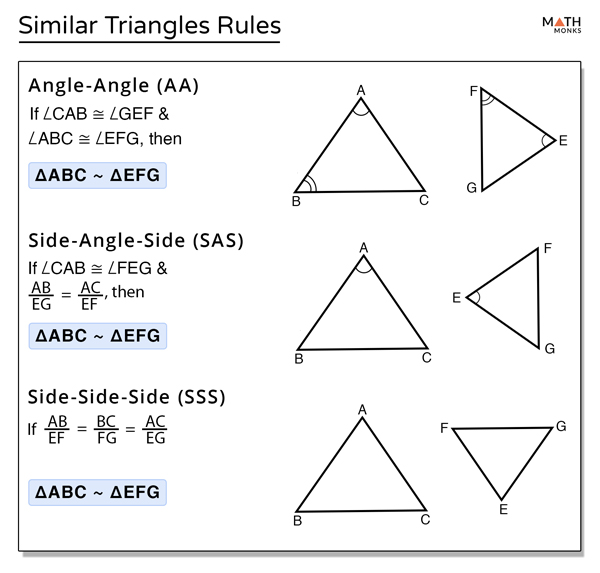
\includegraphics[scale=.7]{Similar-Triangles-Rules.jpg}
\subsection{Properties of similar triangles}
\begin{itemize}
    \item Ratio of corresponding sides
    \item Equal angles
\end{itemize}
\pagebreak
\section{Homothety}
\begin{minipage}{.6\linewidth}
    \subsection{Definition}
    A transformation determined by having a point of origin (O), and a ratio of which points from the origin are scaled to.
    \subsection{Properties}
    \begin{itemize}
        \item Shapes will be similar, not congruent, with only its size varying.
        \item The ratio is a set value and applies to all points in relation to the origin.
        \item (Referencing Figure 4.1) DC is parallel to D’C’. This applies to all other points and their corresponding points that have been scaled from the origin by a set factor.
        \item All angles remain unchanged and the ratio between two line segments stays constant.
        \item If two triangles' sides are parallel to each other, the lines connecting the corresponding points are concurrent.

    \end{itemize}
\end{minipage}
\hfill
\begin{minipage}{.4\linewidth}
    

\tikzset{every picture/.style={line width=0.75pt}} %set default line width to 0.75pt        

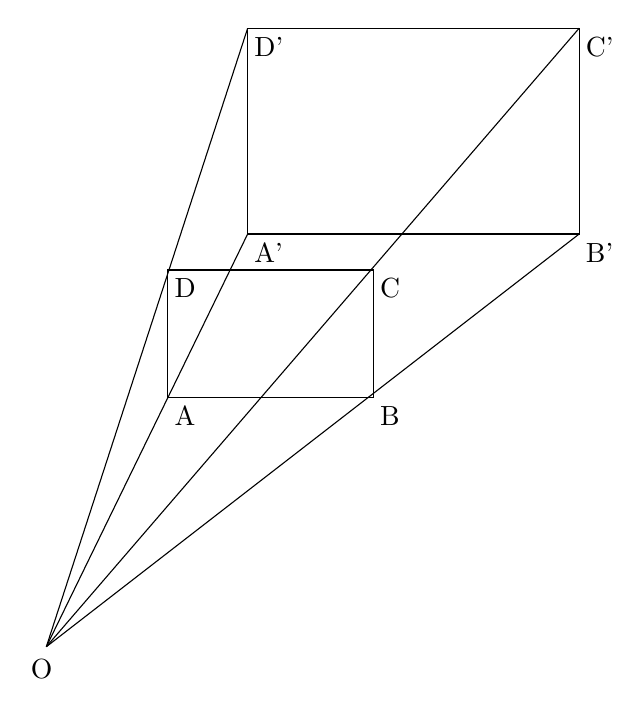
\begin{tikzpicture}[x=0.75pt,y=0.75pt,yscale=-1,xscale=1]
%uncomment if require: \path (0,585); %set diagram left start at 0, and has height of 585

%Straight Lines [id:da4132833494130175] 
\draw    (167.72,164.97) -- (70.72,462.97) ;
%Shape: Rectangle [id:dp6875266857372686] 
\draw   (167.72,164.97) -- (327.44,164.97) -- (327.44,264.11) -- (167.72,264.11) -- cycle ;
%Shape: Rectangle [id:dp7612453265856947] 
\draw   (129.22,281.47) -- (228.22,281.47) -- (228.22,342.92) -- (129.22,342.92) -- cycle ;
%Straight Lines [id:da04306499360890603] 
\draw    (327.44,164.97) -- (70.72,462.97) ;
%Straight Lines [id:da007459425035728939] 
\draw    (70.72,462.97) -- (167.72,264.11) ;
%Straight Lines [id:da3006436753628292] 
\draw    (327.44,264.11) -- (70.72,462.97) ;

% Text Node
\draw (131.22,345.92) node [anchor=north west][inner sep=0.75pt]   [align=left] {A};
% Text Node
\draw (62,467.83) node [anchor=north west][inner sep=0.75pt]   [align=left] {O};
% Text Node
\draw (230.22,345.92) node [anchor=north west][inner sep=0.75pt]   [align=left] {B};
% Text Node
\draw (230.22,284.47) node [anchor=north west][inner sep=0.75pt]   [align=left] {C};
% Text Node
\draw (131.22,284.47) node [anchor=north west][inner sep=0.75pt]   [align=left] {D};
% Text Node
\draw (169.72,267.11) node [anchor=north west][inner sep=0.75pt]   [align=left] {A'};
% Text Node
\draw (329.44,267.11) node [anchor=north west][inner sep=0.75pt]   [align=left] {B'};
% Text Node
\draw (329.44,167.97) node [anchor=north west][inner sep=0.75pt]   [align=left] {C'};
% Text Node
\draw (169.72,167.97) node [anchor=north west][inner sep=0.75pt]   [align=left] {D'};


\end{tikzpicture}

\end{minipage}

\section{Quadrilaterals}
\subsection{Parallelogram}


\tikzset{every picture/.style={line width=0.75pt}} %set default line width to 0.75pt        

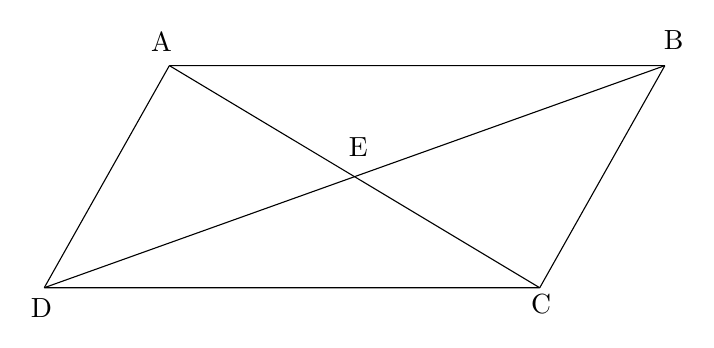
\begin{tikzpicture}[x=0.75pt,y=0.75pt,yscale=-1,xscale=1]
%uncomment if require: \path (0,585); %set diagram left start at 0, and has height of 585

%Straight Lines [id:da35942028032833306] 
\draw    (145,123) -- (383.72,123.02) ;
%Straight Lines [id:da3689932854393849] 
\draw    (145,123) -- (84.72,230.02) ;
%Straight Lines [id:da7016891267736529] 
\draw    (383.72,123.02) -- (323.44,230.04) ;
%Straight Lines [id:da28165775722869] 
\draw    (84.72,230.02) -- (323.44,230.04) ;
%Straight Lines [id:da026398831619073082] 
\draw    (145,123) -- (323.44,230.04) ;
%Straight Lines [id:da6897847573152873] 
\draw    (84.72,230.02) -- (383.72,123.02) ;

% Text Node
\draw (135,106) node [anchor=north west][inner sep=0.75pt]   [align=left] {A};
% Text Node
\draw (382,105) node [anchor=north west][inner sep=0.75pt]   [align=left] {B};
% Text Node
\draw (318,232) node [anchor=north west][inner sep=0.75pt]   [align=left] {C};
% Text Node
\draw (77,234) node [anchor=north west][inner sep=0.75pt]   [align=left] {D};
% Text Node
\draw (230.22,156.52) node [anchor=north west][inner sep=0.75pt]   [align=left] {E};


\end{tikzpicture}

\subsubsection{Definition}
A quadrilateral with both opposite sides parallel to each other.
\subsubsection{Properties}
\begin{itemize}
    \item Opposite side lengths are congruent
    \item When drawing a line between the opposite points, the intersections are midpoints for both lines (AE = EC, therefore E is the midpoint of AC. BE = ED, therefore…).
    \item Angle BAC is the same as ACD (internal angle theorem). This is also the same with angles DAC and ACB. 
\end{itemize}
\subsection{Rhombus}
\subsubsection{Definition}
A parallelogram with congruent side lengths for all four sides.
\subsubsection{Properties}
Same properties as a parallelogram, except all side lengths are the same, all the internal lines are the same, and the intersection of diagnoses forms 90 degree angles.
\subsection{Rectangle}
\subsubsection{Definition}
A parallelogram that has all four angles being 90 degrees each.
\subsubsection{Properties}
\begin{itemize}
    \item Has four sides and four vertices.
    \item Opposite sides are equal.
    \item Opposite sides are parallel.
    \item All four angles are right angles.
    \item Diagonals are equal and bisect each other.
\end{itemize}

\subsection{Square}
\subsubsection{Definition}
A rhombus with each angle being 90 degrees to each other.
\subsubsection{Properties}
\begin{itemize}
    \item Properties of rectangle.
    \item Properties of rhombus.

\end{itemize}
\pagebreak

\section{Midpoint}
\subsection{Midpoint of a right triangle}



\tikzset{every picture/.style={line width=0.75pt}} %set default line width to 0.75pt        

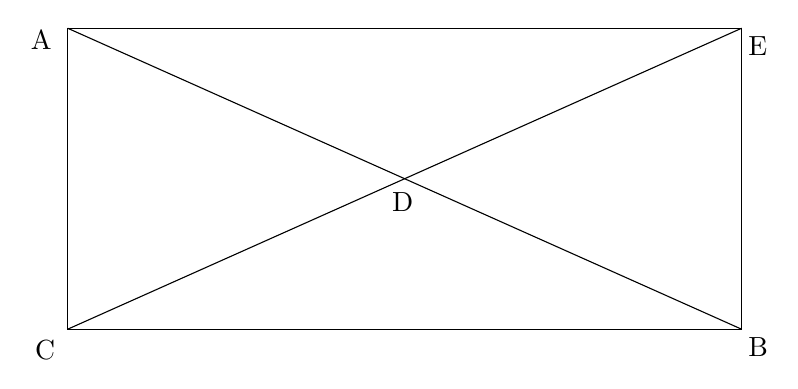
\begin{tikzpicture}[x=0.75pt,y=0.75pt,yscale=-1,xscale=1]
%uncomment if require: \path (0,585); %set diagram left start at 0, and has height of 585

%Shape: Rectangle [id:dp5312133262353695] 
\draw   (100,101) -- (424.72,101) -- (424.72,246.02) -- (100,246.02) -- cycle ;
%Straight Lines [id:da961946909589342] 
\draw    (100,101) -- (424.72,246.02) ;
%Straight Lines [id:da1805570337034097] 
\draw    (424.72,101) -- (100,246.02) ;

% Text Node
\draw (81,101) node [anchor=north west][inner sep=0.75pt]   [align=left] {A};
% Text Node
\draw (426.72,249.02) node [anchor=north west][inner sep=0.75pt]   [align=left] {B};
% Text Node
\draw (83,250) node [anchor=north west][inner sep=0.75pt]   [align=left] {C};
% Text Node
\draw (255,179) node [anchor=north west][inner sep=0.75pt]   [align=left] {D};
% Text Node
\draw (426.72,104) node [anchor=north west][inner sep=0.75pt]   [align=left] {E};


\end{tikzpicture}\\
By rotating $ABC$ 180 degrees on point $D$, a rectangle can be created. The properties of a rectangle states that all internal line segments ($AD$, $CD$, $BD$, and $ED$) are all congruent. Therefore, the midpoint of a right triangle creates $AD$, $CD$, and $BD$, which all have the same side lengths.

\subsection{Midsegment}


\tikzset{every picture/.style={line width=0.75pt}} %set default line width to 0.75pt        

\begin{tikzpicture}[x=0.75pt,y=0.75pt,yscale=-1,xscale=1]
%uncomment if require: \path (0,585); %set diagram left start at 0, and has height of 585

%Shape: Polygon [id:ds8535954377607069] 
\draw   (207.14,166.02) -- (424.72,344.29) -- (159.72,345.02) -- cycle ;
%Straight Lines [id:da1323481298728899] 
\draw    (183.43,255.52) -- (315.93,255.15) ;

% Text Node
\draw (199,146) node [anchor=north west][inner sep=0.75pt]   [align=left] {A};
% Text Node
\draw (152,351) node [anchor=north west][inner sep=0.75pt]   [align=left] {B};
% Text Node
\draw (421,347) node [anchor=north west][inner sep=0.75pt]   [align=left] {C};
% Text Node
\draw (166,246) node [anchor=north west][inner sep=0.75pt]   [align=left] {D};
% Text Node
\draw (320,242) node [anchor=north west][inner sep=0.75pt]   [align=left] {E};
% Text Node
\draw (211,145) node [anchor=north west][inner sep=0.75pt]   [align=left] {(O)};


\end{tikzpicture}\\
$BC$ is parallel to $DE$ since $D$ and $E$ are extended to $B$ and $C$, respectively, by a factor of twice their original side lengths. When referring back to homothety, point $A$ acts as the origin point, therefore making angle $ADE$ and angle $ABC$ the same. Therefore, $DE$ and $BC$ are parallel.

\pagebreak
\section{Problems}
\subsection{Problem}
The quadrilateral formed by joining midpoint of a quadrilateral is a parallelogram.


\tikzset{every picture/.style={line width=0.75pt}} %set default line width to 0.75pt        

\begin{tikzpicture}[x=0.75pt,y=0.75pt,yscale=-1,xscale=1]
%uncomment if require: \path (0,585); %set diagram left start at 0, and has height of 585

%Shape: Polygon [id:ds11098710636502895] 
\draw   (263.72,80.02) -- (472.72,246.02) -- (196.72,453.02) -- (132.72,190.02) -- cycle ;
%Straight Lines [id:da2616559228752324] 
\draw    (198.22,135.02) -- (368.22,163.02) ;
%Straight Lines [id:da8368491190119953] 
\draw    (164.72,321.52) -- (334.72,349.52) ;
%Straight Lines [id:da6891842269917876] 
\draw    (198.22,135.02) -- (164.72,321.52) ;
%Straight Lines [id:da9229584938155542] 
\draw    (368.22,163.02) -- (334.72,349.52) ;
%Straight Lines [id:da3491121859206272] 
\draw    (263.72,80.02) -- (196.72,453.02) ;
%Straight Lines [id:da2004057111959674] 
\draw    (132.72,190.02) -- (472.72,246.02) ;

% Text Node
\draw (119,184) node [anchor=north west][inner sep=0.75pt]   [align=left] {A};
% Text Node
\draw (260,62) node [anchor=north west][inner sep=0.75pt]   [align=left] {B};
% Text Node
\draw (475,238) node [anchor=north west][inner sep=0.75pt]   [align=left] {C};
% Text Node
\draw (189,458) node [anchor=north west][inner sep=0.75pt]   [align=left] {D};
% Text Node
\draw (183,119) node [anchor=north west][inner sep=0.75pt]   [align=left] {E};
% Text Node
\draw (371,148) node [anchor=north west][inner sep=0.75pt]   [align=left] {F};
% Text Node
\draw (336.72,352.52) node [anchor=north west][inner sep=0.75pt]   [align=left] {G};
% Text Node
\draw (152,324) node [anchor=north west][inner sep=0.75pt]   [align=left] {H};


\end{tikzpicture}\\
To prove that $EFGH$ is a parallelogram, one can view point $A$ as a point of origin for homothety. As $AE$ is and $AH$ are doubled to become $AB$ and $AD$, respectively, angle $AHE$ and $ADB$ are the same (ref. 4.2, homothety). Thus, $HE$ and $DB$ are parallel. This analysis can be applied to the three other points (point $B$, $C$, and $D$), where these points are viewed as the point of origin. Therefore, $EH$ and $FG$ can be proven as parallel, and so can $EF$ and $HG$.
\pagebreak
\subsection{Problem}
Given equilateral $\triangle ABC$, extend $BC$ to $D$ and $BA$ to $E$ to let $AE = BD$. Join $CE$ and $DE$. Prove $\triangle ECD =\triangle EDC$.


\tikzset{every picture/.style={line width=0.75pt}} %set default line width to 0.75pt        

\begin{tikzpicture}[x=0.75pt,y=0.75pt,yscale=-1.5,xscale=1.5]
%uncomment if require: \path (0,585); %set diagram left start at 0, and has height of 585

%Shape: Triangle [id:dp5521074684041429] 
\draw   (148.36,150) -- (184.72,216.02) -- (112,216.02) -- cycle ;
%Shape: Triangle [id:dp633221432917475] 
\draw   (205.36,46.51) -- (298.72,216.02) -- (112,216.02) -- cycle ;
%Shape: Triangle [id:dp10333690512719018] 
\draw   (262.36,150) -- (298.72,216.02) -- (226,216.02) -- cycle ;
%Straight Lines [id:da27829047011923613] 
\draw    (184.72,216.02) -- (205.36,46.51) ;
%Straight Lines [id:da23015331486347979] 
\draw    (205.36,46.51) -- (226,216.02) ;

% Text Node
\draw (134,136) node [anchor=north west][inner sep=0.75pt]   [align=left] {A};
% Text Node
\draw (103,221) node [anchor=north west][inner sep=0.75pt]   [align=left] {B};
% Text Node
\draw (175,219) node [anchor=north west][inner sep=0.75pt]   [align=left] {C};
% Text Node
\draw (218,218) node [anchor=north west][inner sep=0.75pt]   [align=left] {D};
% Text Node
\draw (291,220) node [anchor=north west][inner sep=0.75pt]   [align=left] {F};
% Text Node
\draw (203,27) node [anchor=north west][inner sep=0.75pt]   [align=left] {E};


\end{tikzpicture}\\
To prove $\angle ECD =\angle EDC$, extend line $BD$ by a length of $BC$, to create the new point $F$. Connect point $E$ to $F$, to create triangle $EFB$. Since $AE = BD, AE = CF = BD. $
Therefore,$ BE = BA + AE = BC + CF = BF$. Knowing that $EB$ and $BF$ have the same side lengths, and intersect at an angle of 60 degrees, one can conclude that $EFB$ is an equilateral triangle ($EFB$ is an isosceles, therefore angle $BEF$ and $EFB$ must equal to 
(180 - 60)/2 = 120 / 2 = 60 degrees, therefore equilateral). 
Once that has been proven, one can prove that $BCE$ and $FDE$ are the same due to SAS, therefore proving that $\angle ECD$ and $\angle EDC$ are congruent.
\pagebreak
\subsection{Problem}
In quadrilateral $ABCD$ with $AD = BC$, $E$ and $F$ are midpoints on $AB$ and $CD$, respectively. $EF$ meets $AD$ at $G$, meets $BC$ at $H$. Prove $\angle DGF = \angle CHF$.


\tikzset{every picture/.style={line width=0.75pt}} %set default line width to 0.75pt        

\begin{tikzpicture}[x=0.75pt,y=0.75pt,yscale=-1,xscale=1]
%uncomment if require: \path (0,585); %set diagram left start at 0, and has height of 585

%Straight Lines [id:da6741940764413128] 
\draw    (136,357) -- (457.72,358.02) ;
%Straight Lines [id:da6351245694924745] 
\draw    (331.72,54.02) -- (136,357) ;
%Straight Lines [id:da40106442921838736] 
\draw    (331.72,54.02) -- (296.86,357.51) ;
%Straight Lines [id:da39306377315538366] 
\draw    (323.72,124.02) -- (457.72,358.02) ;
%Straight Lines [id:da04848886360165583] 
\draw    (235.72,200.02) -- (379.72,220.02) ;
%Straight Lines [id:da6859886517881486] 
\draw    (235.72,200.02) -- (457.72,358.02) ;
%Straight Lines [id:da8545909102904259] 
\draw    (314,212) -- (355.72,287.02) ;
%Straight Lines [id:da37879152074454514] 
\draw    (296.86,357.51) -- (355.72,287.02) ;

% Text Node
\draw (127,363) node [anchor=north west][inner sep=0.75pt]   [align=left] {A};
% Text Node
\draw (459.72,361.02) node [anchor=north west][inner sep=0.75pt]   [align=left] {B};
% Text Node
\draw (380,202) node [anchor=north west][inner sep=0.75pt]   [align=left] {C};
% Text Node
\draw (221,184) node [anchor=north west][inner sep=0.75pt]   [align=left] {D};
% Text Node
\draw (290,364) node [anchor=north west][inner sep=0.75pt]   [align=left] {E};
% Text Node
\draw (301,190) node [anchor=north west][inner sep=0.75pt]   [align=left] {F};
% Text Node
\draw (327,113) node [anchor=north west][inner sep=0.75pt]   [align=left] {H};
% Text Node
\draw (321,36) node [anchor=north west][inner sep=0.75pt]   [align=left] {G};
% Text Node
\draw (358,268) node [anchor=north west][inner sep=0.75pt]   [align=left] {M};


\end{tikzpicture}\\
To prove $\angle DGF = \angle  CHF$, a reference line has to be drawn from point $D$ to point $B$, with point $M$ as the midpoint of $DB$.\\
Then, connect point $F$ to $M$, and $E$ to $M$. \\
When viewing point $B$ as the point of origin $(O)$, lines $EM$ and $AD$ can be viewed as parallel lines, with $EM$ being half of the length of $AD$ because the distance between $OD$ is double of $OM$ (ref. 4.2., Homothety).\\
Apply this analysis but onto point $D$ as the origin point, thus proving $FM$ is both parallel and half the length of $CB$.\\
Since $FM$ and $EM$ are the same lengths, $FME$ is an isosceles triangle with $\angle EFM =\angle MEF$.\\
$BH$ and $HF$ are parallel lines that intersect $EH$, therefore $\angle CHF = \angle MFE$.\\
$DG$ and $EM$ are parallel lines that intersect with $EG$, therefore $\angle DGF = \angle GEM$ (Alternate Interior Angle theorem).\\
Therefore, $\angle \mathrm{DGF}=\angle \mathrm{FEM}=\angle \mathrm{EFM}=\angle \mathrm{FHC} \Rightarrow \angle \mathrm{DGF}=\angle \mathrm{FHC}$.

\end{document}